\section{Introduction}
This document describes the side-channel characterization of a secure AES encryption implementation. 
We perform this study on the ChipWhisperer target based on a STM32F303RCT7 chip (using a Cortex-M4 core).
Using the ChipWhisperer as a board for side-channel characterization
is explained by an easy access to power consumption and clean signal acquisition chain. Furthermore,
this board natively supports the \emph{undercloking} of the Cortex-M4 target using an external
oscillator: slowing down the core frequency to 4 MHz allows to use reasonable sampling rates during
the acquisition.

This evaluation was performed on power consumption traces captured through an oscilloscope, sampling $100.000.000$ samples by second. The obtained traces consist in $2.000.000$ samples, encompassing the whole AES implementation. 
Figure \ref{fig:sample_trace} shows two main steps: the first one is the pre-processing, and the second one is the execution of the raw AES rounds. More details are given in Section \ref{sec:secured_aes}.


\begin{figure}[h!]
  \centering 
  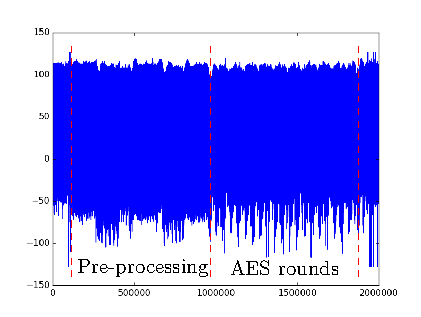
\includegraphics[scale=1]{figures/sample_traces_2M_label.pdf}
  \caption{Power consumption trace of the AES encryption.}
  \label{fig:sample_trace}
\end{figure}

No resynchronization step has been performed on these traces. Nonetheless, visual inspection indicates that no significant desynchronization occurs. To illustrate this, Figure~\ref{fig:3_traces} displays a temporal zoom on three different traces.

\begin{figure}[h]
	\centering 
	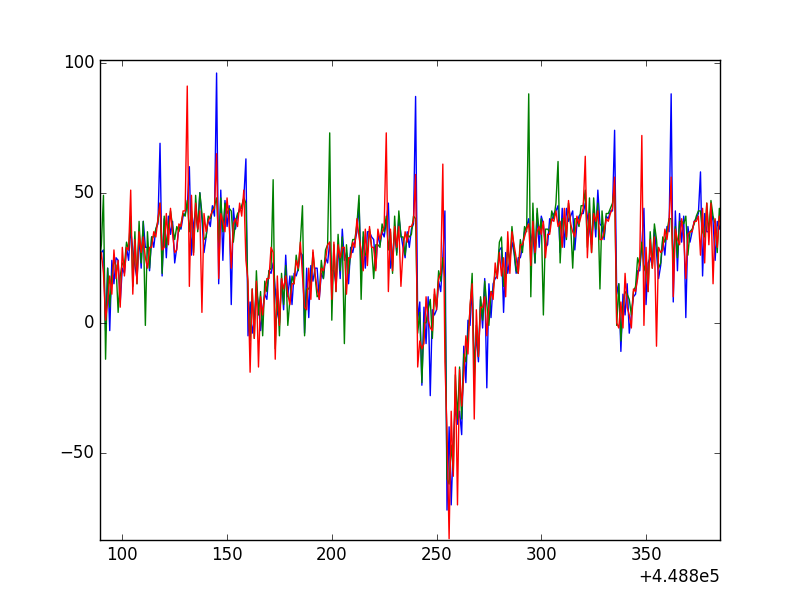
\includegraphics[scale=0.35]{figures/3_traces.png}
	\caption{Three traces on a short temporal window.}
	\label{fig:3_traces}
\end{figure}


A first acquisition campaign of $50.000$ traces of the rolled version (\emph{ie.}, the default version) is used to perform the caracterisation step as well as the first-order resilience assessment.
For the second and third order assessments, we used a second campaign of $100.000$ traces of the unrolled version. The following table summarizes the results.
The analyses are further detailed in the rest of this document.

\begin{figure}[h!]
\centering
\begin{tabular}{|c|c|c|c|c|c|c|}
  \hline
   & \multicolumn{3}{c|}{Known permutation}&\multicolumn{3}{c|}{Unknown permutation}\\
  \hline
  Known    & $\rmult, \rout$ & $\rmult $ &  None & $\rmult,\rout$ & $\rmult $  &  None \\
  \hline
  Order 1& $\approx 1.000$ & $ > 50.000$ & $> 50.000$& $\approx 20.000$ & $ > 50.000$ & > $50.000$\\
  \hline
  Order 2& N/A & $ > 8.000$ & $> 100.000$& N/A & $ > 100.000$ & > $100.000$\\
  \hline
  Order 3& N/A & N/A & $> 100.000$& N/A & N/A & > $100.000$\\
  \hline
\end{tabular}
\caption{Number of traces needed for a successful first-order, second-order, and thirs-order attack, depending on the masks known to the attacker.}
\end{figure}


